\documentclass[a4paper,10pt]{article}
\usepackage[utf8]{inputenc}
\usepackage{graphicx}
\usepackage{geometry}
\usepackage{pdfpages}
\usepackage{afterpage}
\usepackage{scrextend}
\usepackage{pdflscape}
\usepackage{caption}
\title{AIS - Restaurace}
\begin{document}

\renewcommand{\figurename}{Obrázek}
\newcommand\textbox[1]{
	\parbox{.5\textwidth}{#1}
}

% === FRONT PAGE ===
\thispagestyle{plain}
	\newgeometry{left=2cm,right=2cm,top=1.5cm}
	\pagenumbering{gobble}
	\begin{center}
		\Huge
		VYSOKÉ UČENÍ TECHNICKÉ V BRNĚ \\
			\vspace{\stretch{0.150}}


	
\includegraphics[width=\textwidth]{resources/fit-logo.pdf}
			\vspace{\stretch{0.300}}



		\Large{Projekt do předmětu AIS \\ ~ \\}
		
		\LARGE
		\textsc{Prvotní analýza a plán projektu}
			\vspace{\stretch{0.618}}

	\end{center}

	\noindent \textbox{18. října, 2018} \textbox{\hfill \textbf{Autoři:}  Daniel Dušek ~~(xdusek21) ~~~}
	\noindent \textbox{\hfill} \textbox{\hfill Filip Kalous ~~~(xkalou03) ~~~}
	\noindent \textbox{\hfill} \textbox{\hfill Anna Popková (xpopko00)~~~}

	\clearpage
	\restoregeometry

\newpage

\normalsize

\newpage
\thispagestyle{empty}
\section*{Neformální specifikace projektu}
Středně velká restaurace potřebuje informační systém, který usnadní komunikaci a~synchronizaci mezi personálem kuchyně, obsluhy, kanceláří a~zákazníky. Zejména pak pro řešení rezervací stolů, salónku, přijatých a~vyhotovených objednávek jídla.

Restaurace sestává ze čtyř logických částí. Kuchyně, část ve které se pohybuje obsluha, místa v~restauraci a~kancelář. Systém by měl umožnit pracovníkům obsluhy předat informaci o~objednaných jídlech do kuchyně a~následně pak pracovníkům kuchyně zobrazit objednaná jídla a~upravovat stav jejich vyhotovení.

Běžný zákazník restaurace přijde do styku pouze s~webovou aplikací, která systém rozšiřuje, a~umožňuje zarezervovat si konkrétní místo u~stolu, stůl, popřípadě celý salónek v~uživatelem zvoleném termínu. Prostřednictvím rezervačního rozhraní si může také zákazník zobrazit kdy jsou a~nejsou místa k~rezervaci volná. Uživatel dále může svou rezervaci stornovat. Nezávisle k~rezervaci může také poslat zpětnou vazbu majiteli restaurace prostřednictvím formuláře dostupného v~na systému nezávislé webové aplikaci.

Pracovníci obsluhy si mohou zobrazovat existující rezervace a~stav stolů a~salónků. Dále mohou prostřednictvím systému označovat stoly jako volné a~obsazené. Obsluha dále může zadávat do systému objednávky pro kuchyň a~sledovat stav těchto objednávek.

Kuchyňský personál může zobrazovat objednaná jídla a~měnit jejich stav podle toho, jak se daří jejich vyhotovení. Kuchyňský personál může žádat kancelář o~dozásobení konkrétním typem suroviny, která v~kuchyni chybí. Dále může kuchyňský personál editovat denní menu restaurace.

Kancelářský personál potvrzuje, zamítá a~ruší prostřednictvím systému rezervace, které vytvořili zákazníci skrze webovou aplikaci. Systém si tyto vytvořené rezervace v~pravidelných intervalech stahuje.

Vedení restaurace má k~dispozici jakoukoliv operaci, kterou má k~dispozici libovolný aktér v~systému.


\section*{Prvotní analýza požadavků}

Dle neformální specifikace budou systém používat dvě hlavní skupiny aktérů:
\begin{enumerate}
\item \textbf{Aktér Zákazník}:
Jeho cílem je zprostředkovaně pomocí webové aplikace uskutečnit rezervaci v~restauraci, prohlídnout si aktuální menu a~případně aktuální obsazenost restaurace.
\item \textbf{Aktér Personál}:
Jedná se o~abstraktního aktéra spojeného s~obecnými akcemi jako je zobrazení rezervací a~aktuálníh obsazenosti restaurace. V~kontextu vztahu generalizace-specializace jsou specializací této skupiny následující potomci:
\begin{enumerate}
\item  \textbf{Aktér Kancelář}, který spravuje rezervace vytvořené aktérem Zákazníkem.
\item  \textbf{Aktér Obslužný personál}, který si tyto rezervace může prohlížet, a~který zadává do systému objednávky zákazníků sedících přímo v~restauraci.
\item  \textbf{Aktér Kuchyňský personál}, který aktuální objednávky spravuje a~také může podat požadavek na dozásobení chybějící suroviny v~kuchyni.
\end{enumerate}
Nakonec v systému vystupuje speciální \textbf{aktér Vedení}, který má přístup k~jakékoliv akci, ke které mají přístup aktéři spadající pod skupinu Personál.
\end{enumerate}

Vztahy a případy užití jednotlivých aktérů jsou zobrazeny v následujícím diagramu:

Z~implementačního hlediska bude systém pro restauraci realizován jako samostatná aplikace s přístupem k privátní databázi, ke které bude možné získat přístup pouze z~vnitřní sítě restaurace. Související webová aplikace bude informace o~rezervacích, aktuální obsazenosti restaurace a~menu ukládat do oddělené databáze. Tyto informace budou do webové aplikace zasílány zevnitř informačního systému při každé jejich změně. Obráceně pak, informační systém bude získávat v pravidelných intervalech informace o~nových rezervacích a~zobrazovat je pracovníkům v~kanceláři ke zpracování.

\section*{Plán projektu}

Vzhledem ke komplexnosti projektu jsme se rozhodli rozdělit vývoj tohoto systému do tří iterací, kde v~každé iteraci bude přidána určitá klíčová funkcionalita.

V~první iteraci bude systém umět obsloužit požadavky na rezervace a~s~tím spojené operace. V~této fázi v~systému vystupují pouze základní aktéři: Zákazník, Personál a~Vedení.
Případy užití pokryté v~této iteraci zobrazuje obrázek~1.

Ve druhé iteraci budou rozšířeny možnosti rezervací a~dále bude přidána možnost správy objednávek. V~této fázi již v~systému vystupují všichni aktéři.
Funkcionalita pokrytá v~této iteraci je zachycena v diagramu na obrázku~2.

Ve třetí (závěrečné) iteraci jsou vylepšeny možnosti organizace prostoru a~služeb restaurace tak, že bude systém odpovídat diagramu na obrázku~3.

%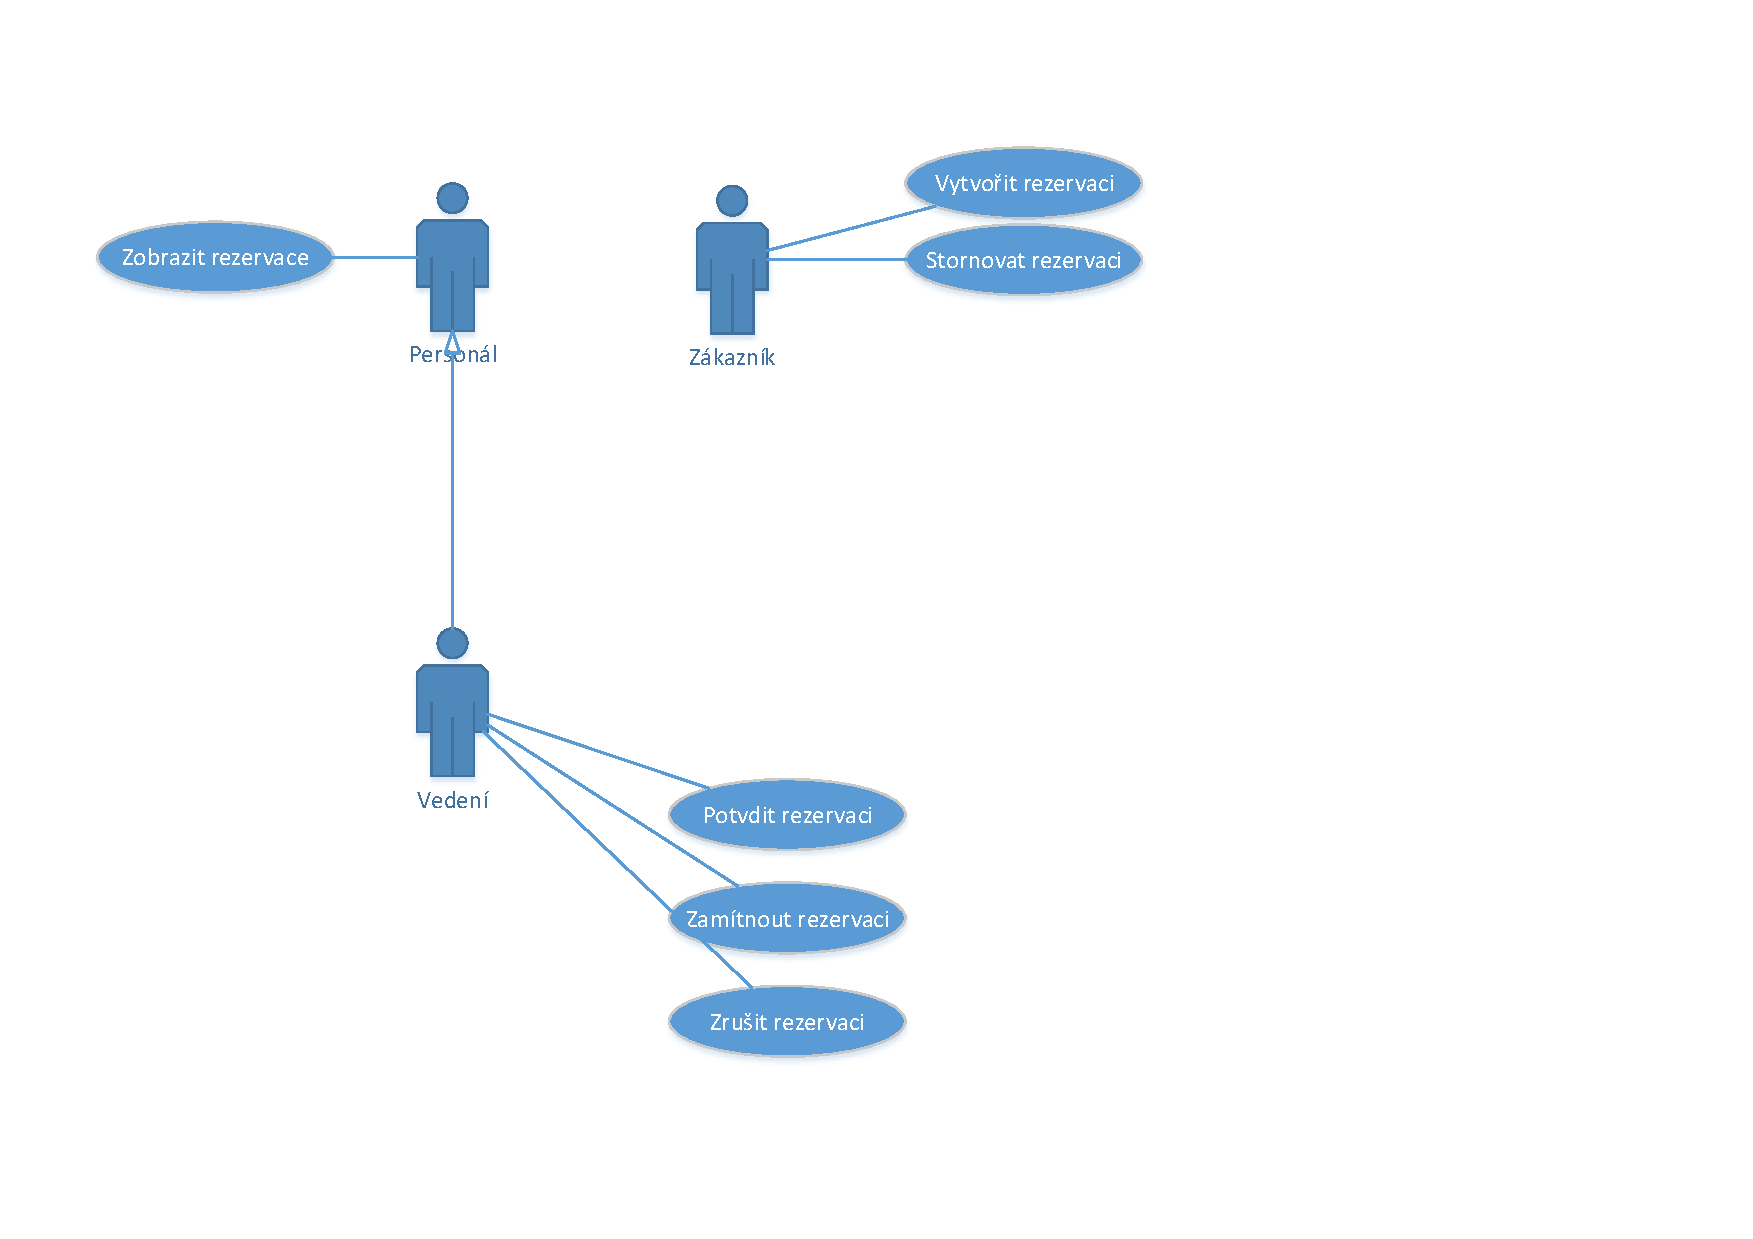
\includegraphics[landscape]{resources/iteration01.pdf}
\begin{center}
\afterpage{
	\pagenumbering{gobble}
	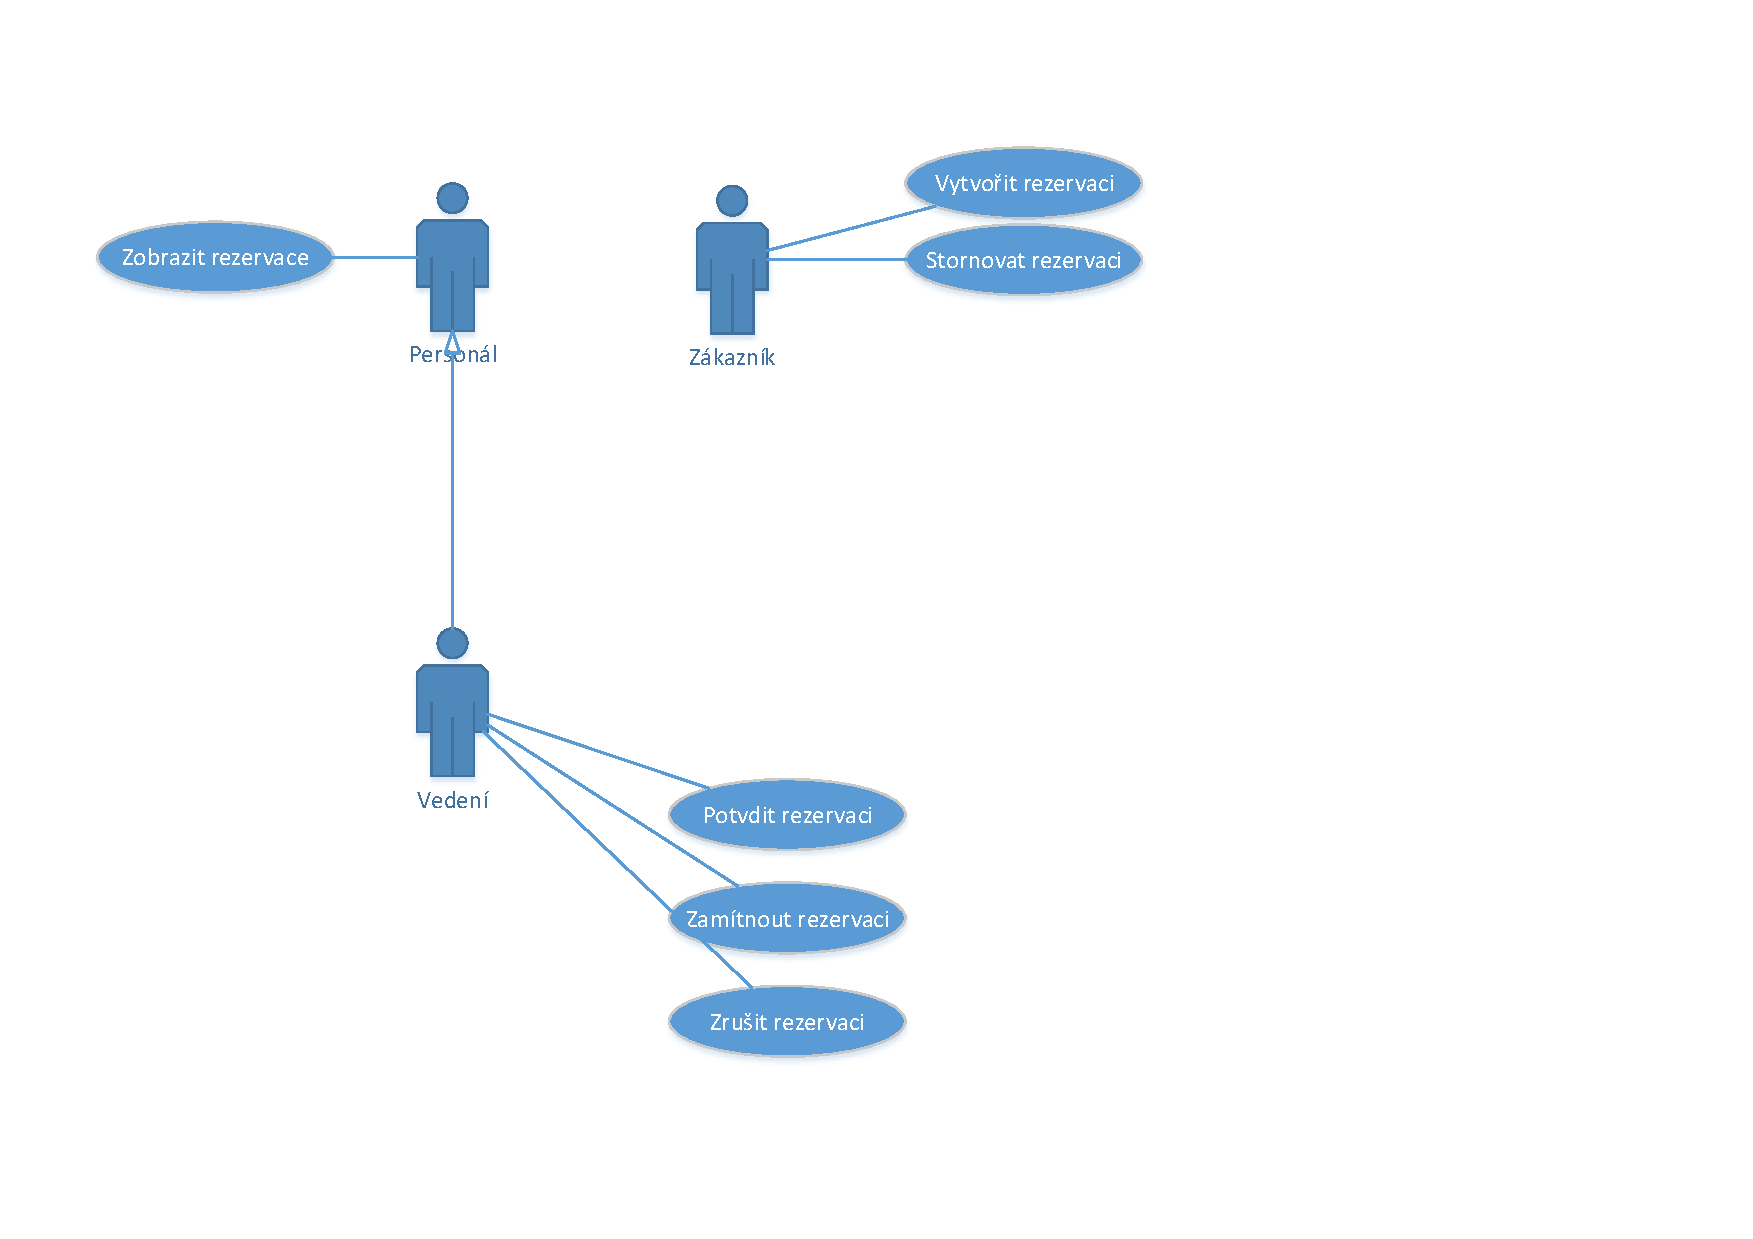
\includepdf[offset=3cm 5cm,pagecommand={
		\thispagestyle{empty}
		\null\vfill
		\captionof{figure}{Diagram použití v první iteraci}}]{resources/iteration01.pdf}
	\label{fig:iteration01}
	\clearpage
	\restoregeometry
}
\end{center}


\begin{landscape}	
	\afterpage{
		
		\pagenumbering{gobble}

		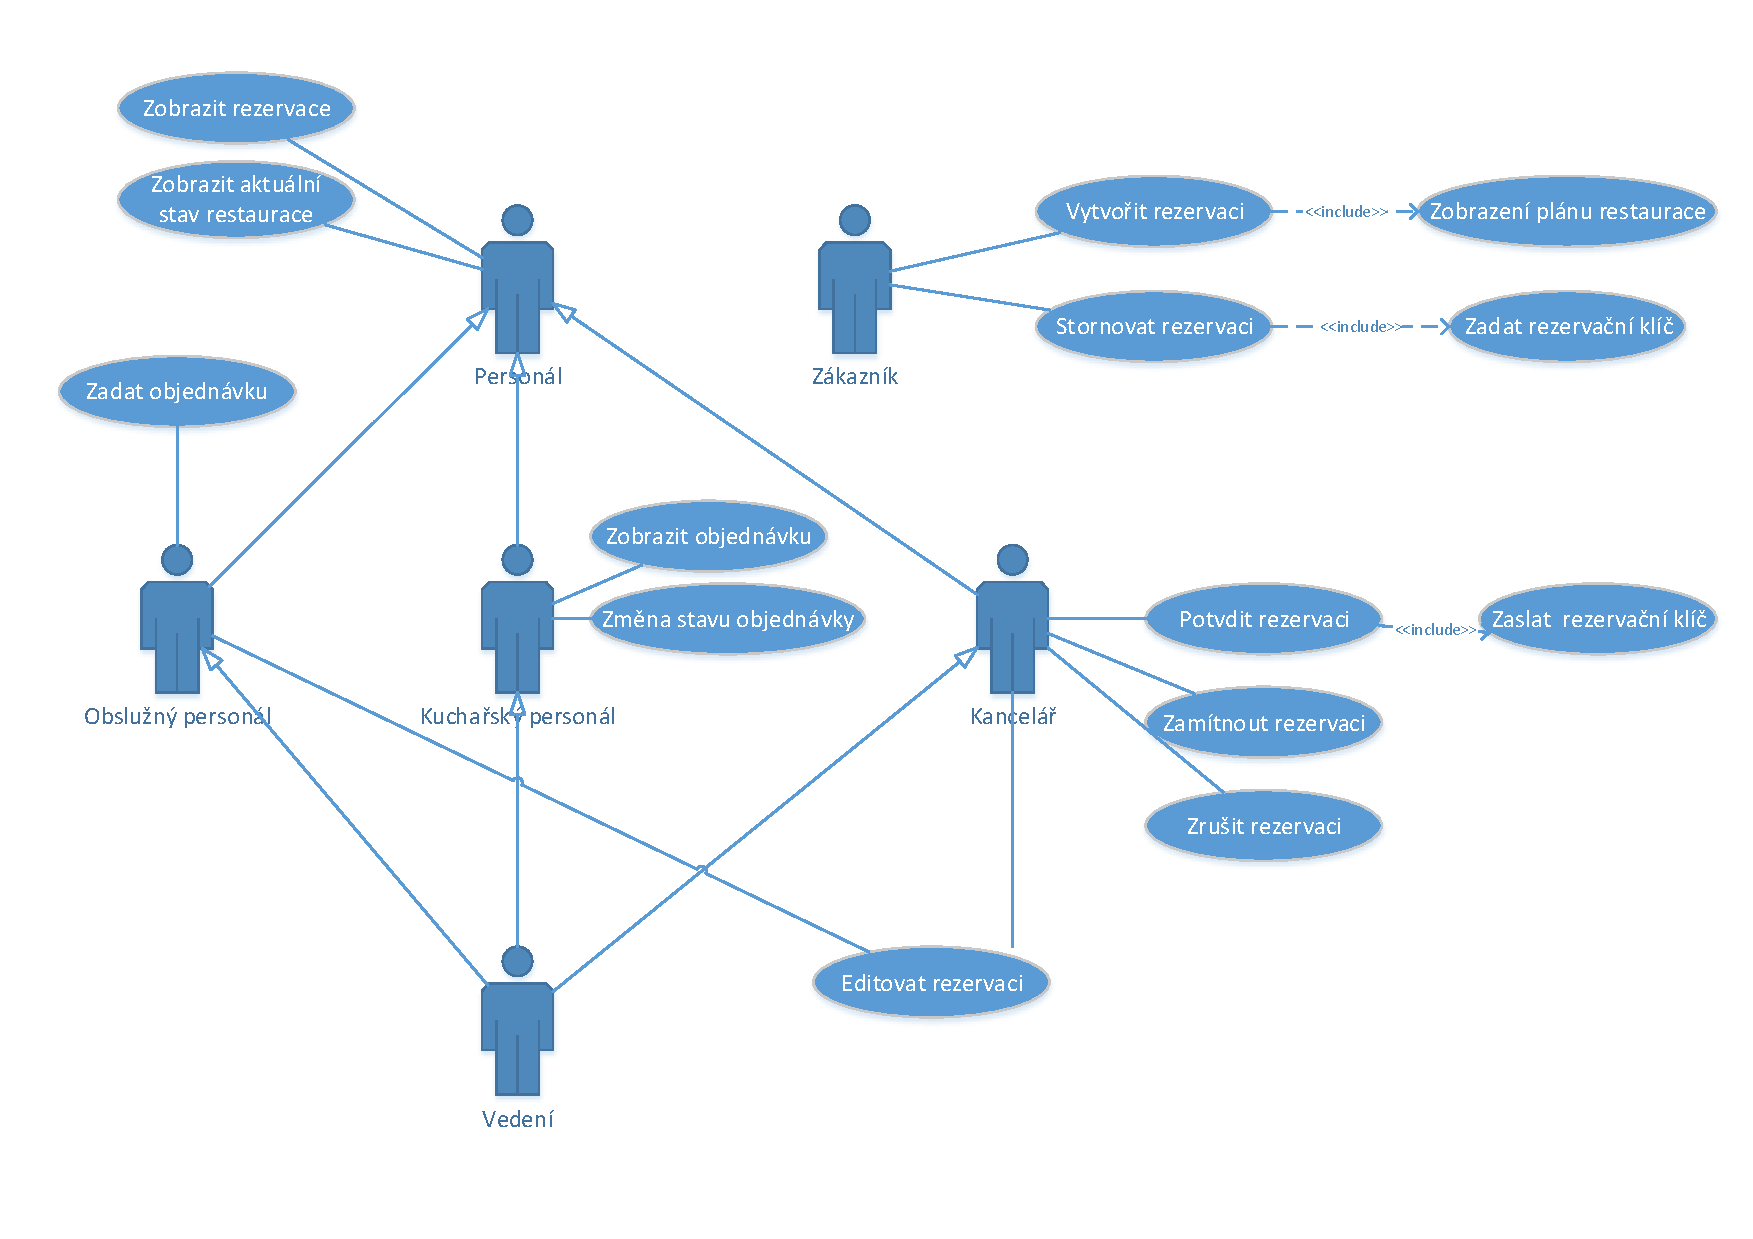
\includepdf[angle=90,scale=0.80,
			pagecommand={
				\thispagestyle{plain}
				\null\vfill
				\captionof{figure}{Diagram použití v druhé iteraci}}]{resources/iteration02.pdf}
		\label{fig:iteration02}
	
		\clearpage
		\restoregeometry
	}
\end{landscape}


\begin{landscape}	
	\afterpage{
			
			\pagenumbering{gobble}

			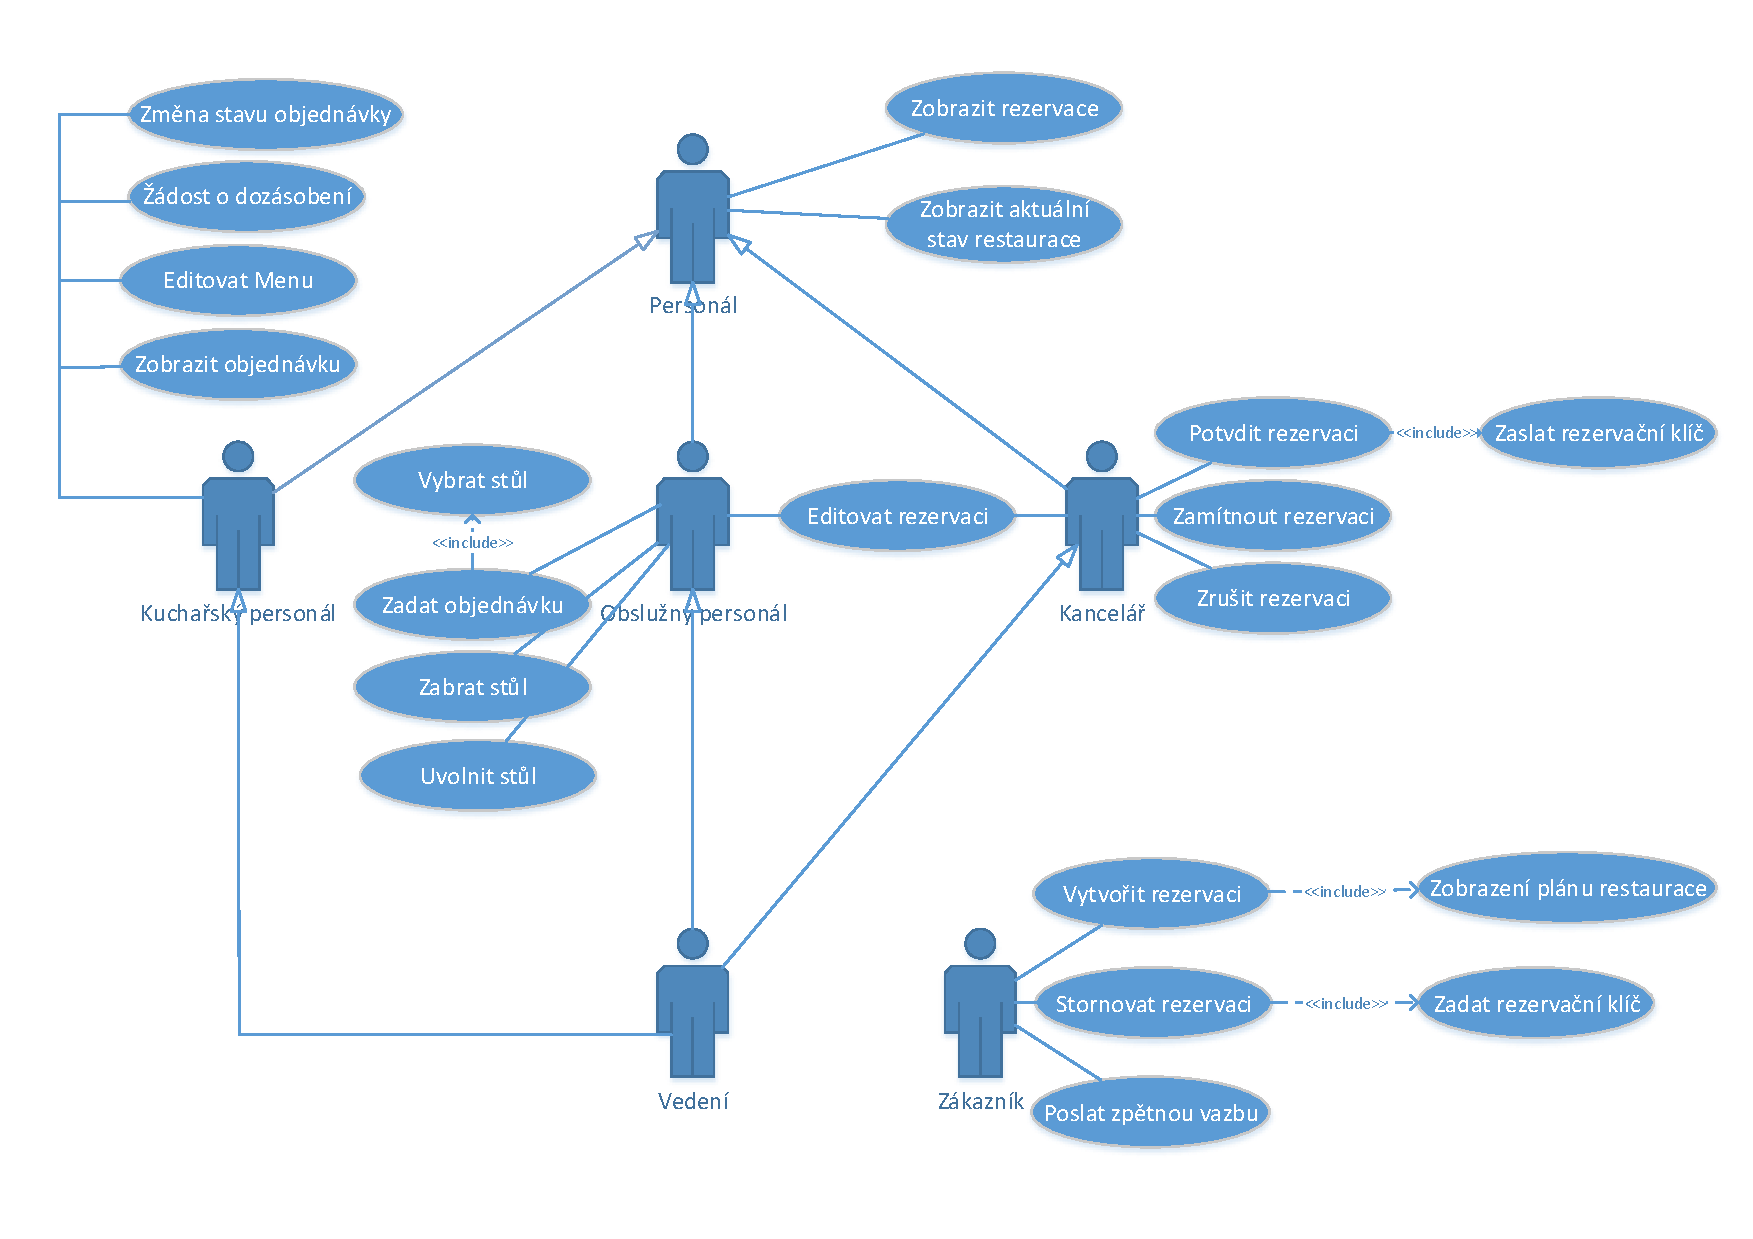
\includepdf[angle=90,scale=0.70,
				pagecommand={
					\thispagestyle{plain}
					\null\vfill
					\captionof{figure}{Diagram použití v třetí iteraci}}]{resources/iteration03.pdf}
			\label{fig:iteration03}
		
			\clearpage
			\restoregeometry
		}
\end{landscape}


\end{document}
